The amazon dataset was the first mandatory dataset. We accomplished getting a score of 72.8\% on kaggle. The high dimensionality is the challenge of this dataset.

\subsection{Characteristics}

\begin{itemize}
\item No missing values
\item 50 different target classes
\item Only rational data
\item 10 000 attributes
\item 750 samples
\end{itemize}

With its 10 000 attributes it is high dimensional.
Therefore Feature Selection is important, but features can not be interpreted by hand, because there are too many.
In order to find good features algorithms from scipy were used as described in section \ref{fig:amazon-feature-selection}.

\subsection{Characteristics of Target value}
The target classes are the different authors of the reviews.
 There are 50 different authors, even though the dataset has a lot of samples there are only a few samples per class.
This is shownn in Figure \ref{fig:amazon-target}. With a minimum of 8 samples written by CFH and a maximum of 21 samples written by Chell. 
On the other hand 10 000 attributes for each sample might be sufficient for classification.

\image{amazon/plots/target.png}{Histogram of the target values}{\label{fig:amazon-target}}

% \begin{figure}[H]
%   \begin{center}
%     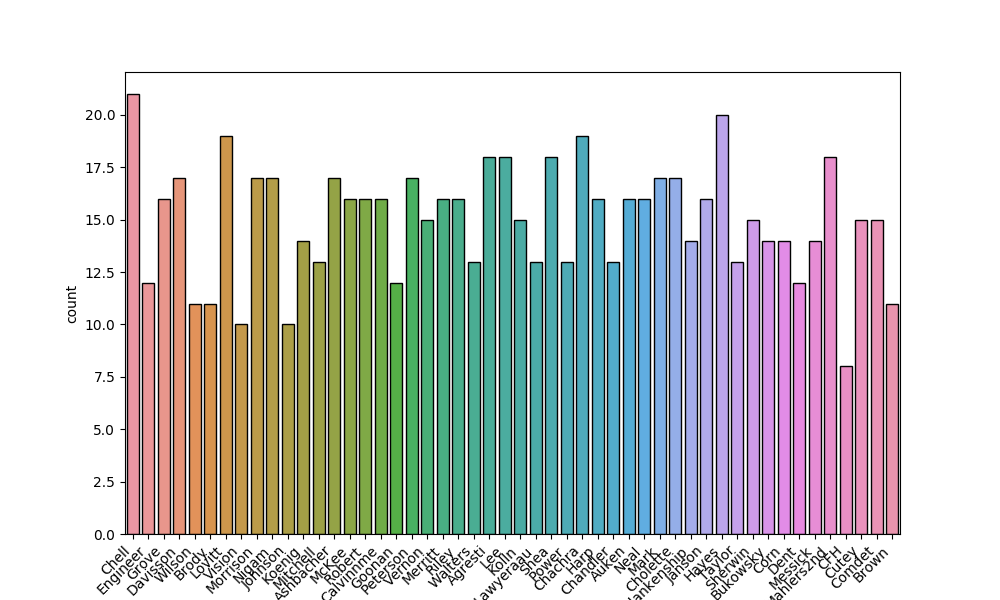
\includegraphics[width=\linewidth]{amazon/plots/target.png}
%     \caption{Histogram of the target values}
%     \label{fig:amazon-target}
%   \end{center}
% \end{figure}


\subsection{Feature selection}
\label{amazon-feature-selection}
Feature selection improves results and reduce the runtime a lot. It was not possible to train the multi layer perceptron without feature selection, because it took over 10 minutes to complete, therefore no comparison without feature selection would be possible. The results are improved by 20-40 percent depending on the classifier. 

Features were selected by SelectKBest and recursive feature elimination and cross-validated selection of the best numbers of features.
SelectKBest performs ${\chi}^2$ test on the samples to retrieve the best features.
As seen in Figure \ref{fig:amazon-feature-selection} at least 1000 features should be used to cross the 55 percent mark, however no difference in performance could be detected between 1000 and 4000 selected features.

\image{amazon/plots/rf_feature_selection.png}{recursive feature selection with random forest tree}{\label{fig:amazon-feature-selection}}

% \begin{figure}[H]
%   \begin{center}
%     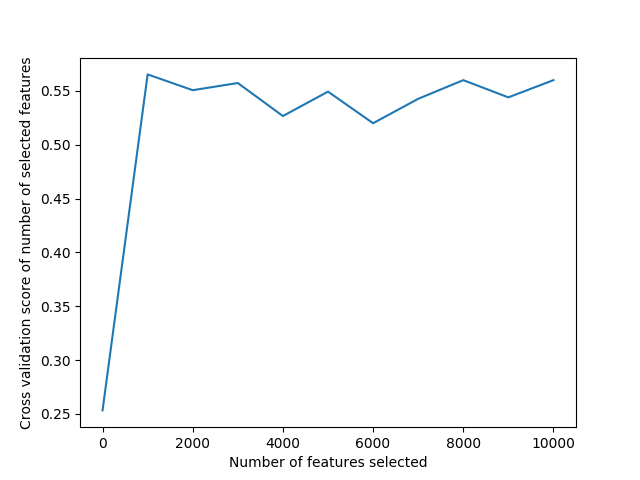
\includegraphics[height=7cm]{amazon/plots/rf_feature_selection.png}
%     \caption{Comparison of different metrics}
%     \label{fig:amazon-feature-selection}
%   \end{center}
% \end{figure}

\subsection{K Nearest Neighbors Classifier}

For K Nearest Neighbours a Grid Search with cross validation was used. The euclidean, chebyshev, manhattan, manhattan and k between 1 and 60 were tested. 
The best k for KNN without preprocessing and all attributes was 10.
The best k for KNN with preprocessing and features selected by recursive feature selection was 15.
K Nearest Neighbors Classifier worked best with weights set to distance, so that the importance of the k neighbors are weighted by their distances to other samples.
This increased results by about 5\%. As seen in Figure \ref{fig:amazon-knn-metric-comparison} the manhattan metric worked best.
The best performance of KNN was 44.13\% which is poor in comparison to random forest and mlp.
This is probably due to the small sample size in comparison to the target class size.
However it evaluated much faster, so first impressions could be derived more quickly.

\image{amazon/plots/knn_metrics.png}{Comparison of knn metrics}{\label{fig:amazon-knn-metric-comparison}}
% \begin{figure}[H]
%   \begin{center}
%     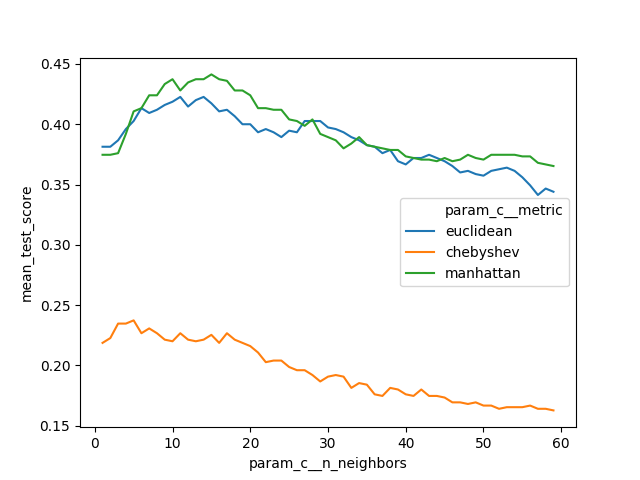
\includegraphics[width=\linewidth]{amazon/plots/knn_metrics.png}
%     \caption{Comparison of different metrics}
%     \label{fig:amazon-knn-metric-comparison}
%   \end{center}
% \end{figure}

Preprocessing with MinMax scalar improved results by around 5\% as seen in figure \ref{fig:amazon-knn-comparison}.
Scaling with mean and variance did lead to better results, but it was not as good as the min max scaler.

\image{amazon/plots/knn_comparison.png}{Comparison of the best estimators with preprocessing and without preprocessing}{\label{fig:amazon-knn-comparison}}

% \begin{figure}[H]
%   \begin{center}
%     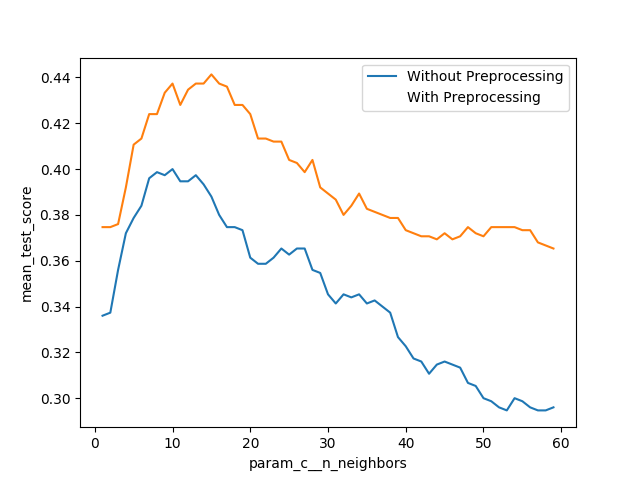
\includegraphics[width=\linewidth]{amazon/plots/knn_comparison.png}
%     \caption{Comparison of the best estimators with preprocessing and without preprocessing}
%     \label{fig:amazon-knn-comparison}
%   \end{center}
% \end{figure}


\subsection{Random Forest Classifier}

As previously described Grid Search with cross validation was used to find the best parameters.
However this initially took too long for all parameters.
So random search with cross validation was used to approximate features first.
Then grid search, with a smaller search space based on the obtained results, was performed.
The best features of Figure \ref{fig:amazon-feature-selection} were used to improve the results even more. 
As seen in Figure \ref{fig:amazon-rf-comparison}, a low maximum features yielded good results, because of the high dimensionality.
With 34 estimators and 30\% max features, a score of 60\% was accomplished which is almost as good as the multi layer perceptron.
However it took significantly longer to evaluate than KNN.

\image{amazon/plots/rf_comparison.png}{Comparison of random forest parameters}{\label{fig:amazon-rf-comparison}}

% \begin{figure}[H]
%   \begin{center}
%     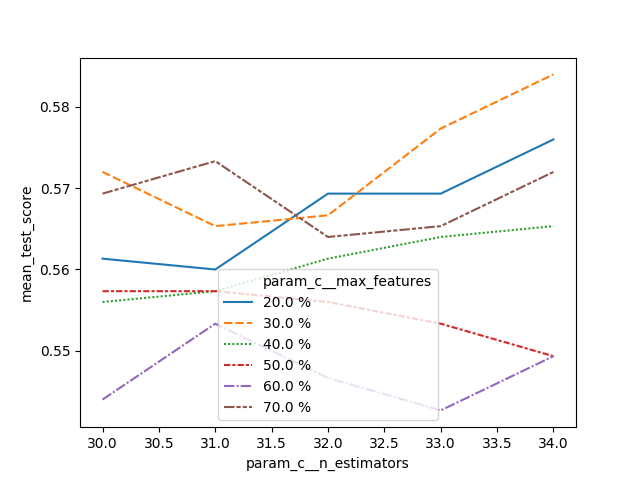
\includegraphics[width=\linewidth]{amazon/plots/rf_comparison.png}
%     \caption{Comparison of the best estimators with preprocessing and without preprocessing}
%     \label{fig:amazon-rf-comparison}
%   \end{center}
% \end{figure}

\subsection{Multi-Layer Perceptron Classifier}

For MLP grid search with a small search space was used, because testing out different hyperparameters is not feasable, because it takes a lot of time.`
As shown in figure \ref{fig:amazon-mlp-comparison} choosing different activation functions does hardly make any difference.
A score of 72.8 \% accuracy was obtained in kaggle by using 2000 selected features with ${\chi}^2$ tests, relu as activation and one hidden layer with 100 neurons.

\image{amazon/plots/mlp_comparison.png}{Comparison of mlp parameters}{\label{fig:amazon-mlp-comparison}}

% \begin{figure}[H]
%   \begin{center}
%     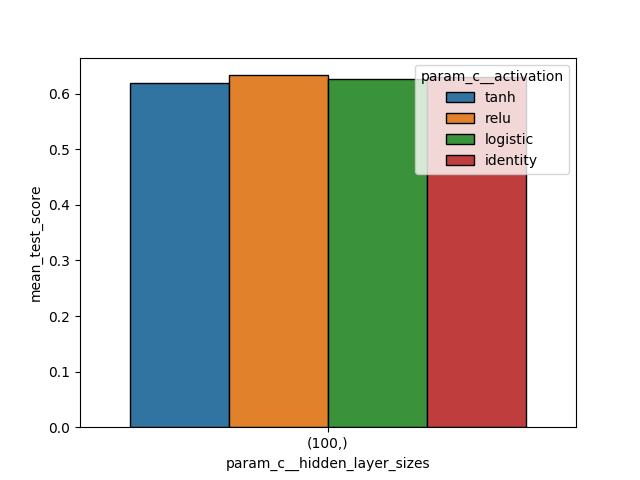
\includegraphics[width=\linewidth]{amazon/plots/mlp_comparison.png}
%     \caption{Comparison of the best estimators with preprocessing and without preprocessing}
%     \label{fig:mlp-comparison}
%   \end{center}
% \end{figure}

\subsection{Conclusion}

Scaling and feature selection improve results quite a bit. While scaling does not affect the random forest classifier, it is important for both k nearest neighbors and the multi layer perceptron. Feature selection is important for all classifiers. Support Vector machines were tried out as well, because they are suited for high dimensional data, but gave a maximum score of 63.46 \%

\begin{table}[ht]
\begin{center}
\begin{tabular}{|l|l|l|}
\hline
                       & Preprocessing & No-Preprocessing \\ \hline
KNeighborsClassifier   & 0.4413        & 0.4000           \\ \hline
RandomForestClassifier & 0.6026        & 0.5840           \\ \hline
MLPClassifier          & 0.6746        & 0.6133           \\ \hline
\end{tabular}
\caption{Comparision of accuracy of different techniques with- and without preprocessing}
\end{center}
\end{table}

Holdout yields different results than cross validation. As cross validation takes a lot of time it is feasable to use them anyways for parameter optimization, but note that their results differ up to 5 \%.

\begin{table}[ht]
\begin{center}
\begin{tabular}{|l|l|l|}
\hline
                       & Holdout & Cross Validation \\ \hline
KNeighborsClassifier   & 0.4066  & 0.4413           \\ \hline
RandomForestClassifier & 0.5333  & 0.5946           \\ \hline
MLPClassifier          & 0.6133  & 0.6746           \\ \hline
\end{tabular}
\caption{Comparision of accuracy of holdout versus cross-validation}
\end{center}
\end{table}

Accuracy is the correct performance metric when evaluating how good this goal was achived. 
Accuracy is the most useful measurement for the amazon dataset, because the most interesting goal is to find out which review is written by which author.
The runtime is the average runtime it took to fit the train data for 10 folds.
The MLP classifier was faster than the random forest tree, because it was simplified in order to run faster and keep it from overfitting.
Other than that knn was the fastest, because it is a lazy learner.

\begin{table}[ht]
\begin{center}
\begin{tabular}{|l|l|l|l|l|l|}
\hline
                       & Accuracy & Precision & Recall & F1     & Runtime (sec) \\ \hline
KNeighborsClassifier   & 0.4333   & 0.3847    & 0.4356 & 0.3805 & 30.987        \\ \hline
RandomForestClassifier & 0.5946   & 0.5400    & 0.5893 & 0.5393 & 481.152       \\ \hline
MLPClassifier          & 0.6986   & 0.6604    & 0.6930 & 0.6522 & 87.990        \\ \hline
\end{tabular}
\caption{Comparision of different performance metrics and runtimes}
\end{center}
\end{table}

